

\documentclass[conference]{IEEEtran}

\usepackage{epstopdf}
\usepackage{graphicx}
\usepackage{epsfig}
\usepackage{listings}
\usepackage{subfigure}



% *** GRAPHICS RELATED PACKAGES ***
%
\ifCLASSINFOpdf
  %\usepackage[pdftex]{graphicx}
  %declare the path(s) where your graphic files are
  % \graphicspath{{../pdf/}{../jpeg/}}
  % and their extensions so you won't have to specify these with
  % every instance of \includegraphics
  % \DeclareGraphicsExtensions{.pdf,.jpeg,.png}
\else
  % or other class option (dvipsone, dvipdf, if not using dvips). graphicx
  % will default to the driver specified in the system graphics.cfg if no
  % driver is specified.
  % \usepackage[dvips]{graphicx}
  % declare the path(s) where your graphic files are
  % \graphicspath{{../eps/}}
  % and their extensions so you won't have to specify these with
  % every instance of \includegraphics
  % \DeclareGraphicsExtensions{.eps}
\fi
% graphicx was written by David Carlisle and Sebastian Rahtz. It is
% required if you want graphics, photos, etc. graphicx.sty is already
% installed on most LaTeX systems. The latest version and documentation can
% be obtained at: 
% http://www.ctan.org/tex-archive/macros/latex/required/graphics/
% Another good source of documentation is "Using Imported Graphics in
% LaTeX2e" by Keith Reckdahl which can be found as epslatex.ps or
% epslatex.pdf at: http://www.ctan.org/tex-archive/info/
%
% latex, and pdflatex in dvi mode, support graphics in encapsulated
% postscript (.eps) format. pdflatex in pdf mode supports graphics
% in .pdf, .jpeg, .png and .mps (metapost) formats. Users should ensure
% that all non-photo figures use a vector format (.eps, .pdf, .mps) and
% not a bitmapped formats (.jpeg, .png). IEEE frowns on bitmapped formats
% which can result in "jaggedy"/blurry rendering of lines and letters as
% well as large increases in file sizes.
%
% You can find documentation about the pdfTeX application at:
% http://www.tug.org/applications/pdftex





% *** MATH PACKAGES ***
%
%\usepackage[cmex10]{amsmath}
% A popular package from the American Mathematical Society that provides
% many useful and powerful commands for dealing with mathematics. If using
% it, be sure to load this package with the cmex10 option to ensure that
% only type 1 fonts will utilized at all point sizes. Without this option,
% it is possible that some math symbols, particularly those within
% footnotes, will be rendered in bitmap form which will result in a
% document that can not be IEEE Xplore compliant!
%
% Also, note that the amsmath package sets \interdisplaylinepenalty to 10000
% thus preventing page breaks from occurring within multiline equations. Use:
%\interdisplaylinepenalty=2500
% after loading amsmath to restore such page breaks as IEEEtran.cls normally
% does. amsmath.sty is already installed on most LaTeX systems. The latest
% version and documentation can be obtained at:
% http://www.ctan.org/tex-archive/macros/latex/required/amslatex/math/





% *** SPECIALIZED LIST PACKAGES ***
%
%\usepackage{algorithmic}
% algorithmic.sty was written by Peter Williams and Rogerio Brito.
% This package provides an algorithmic environment fo describing algorithms.
% You can use the algorithmic environment in-text or within a figure
% environment to provide for a floating algorithm. Do NOT use the algorithm
% floating environment provided by algorithm.sty (by the same authors) or
% algorithm2e.sty (by Christophe Fiorio) as IEEE does not use dedicated
% algorithm float types and packages that provide these will not provide
% correct IEEE style captions. The latest version and documentation of
% algorithmic.sty can be obtained at:
% http://www.ctan.org/tex-archive/macros/latex/contrib/algorithms/
% There is also a support site at:
% http://algorithms.berlios.de/index.html
% Also of interest may be the (relatively newer and more customizable)
% algorithmicx.sty package by Szasz Janos:
% http://www.ctan.org/tex-archive/macros/latex/contrib/algorithmicx/




% *** ALIGNMENT PACKAGES ***
%
%\usepackage{array}
% Frank Mittelbach's and David Carlisle's array.sty patches and improves
% the standard LaTeX2e array and tabular environments to provide better
% appearance and additional user controls. As the default LaTeX2e table
% generation code is lacking to the point of almost being broken with
% respect to the quality of the end results, all users are strongly
% advised to use an enhanced (at the very least that provided by array.sty)
% set of table tools. array.sty is already installed on most systems. The
% latest version and documentation can be obtained at:
% http://www.ctan.org/tex-archive/macros/latex/required/tools/


%\usepackage{mdwmath}
%\usepackage{mdwtab}
% Also highly recommended is Mark Wooding's extremely powerful MDW tools,
% especially mdwmath.sty and mdwtab.sty which are used to format equations
% and tables, respectively. The MDWtools set is already installed on most
% LaTeX systems. The lastest version and documentation is available at:
% http://www.ctan.org/tex-archive/macros/latex/contrib/mdwtools/


% IEEEtran contains the IEEEeqnarray family of commands that can be used to
% generate multiline equations as well as matrices, tables, etc., of high
% quality.


%\usepackage{eqparbox}
% Also of notable interest is Scott Pakin's eqparbox package for creating
% (automatically sized) equal width boxes - aka "natural width parboxes".
% Available at:
% http://www.ctan.org/tex-archive/macros/latex/contrib/eqparbox/





% *** SUBFIGURE PACKAGES ***
%\usepackage[tight,footnotesize]{subfigure}
% subfigure.sty was written by Steven Douglas Cochran. This package makes it
% easy to put subfigures in your figures. e.g., "Figure 1a and 1b". For IEEE
% work, it is a good idea to load it with the tight package option to reduce
% the amount of white space around the subfigures. subfigure.sty is already
% installed on most LaTeX systems. The latest version and documentation can
% be obtained at:
% http://www.ctan.org/tex-archive/obsolete/macros/latex/contrib/subfigure/
% subfigure.sty has been superceeded by subfig.sty.



%\usepackage[caption=false]{caption}
%\usepackage[font=footnotesize]{subfig}
% subfig.sty, also written by Steven Douglas Cochran, is the modern
% replacement for subfigure.sty. However, subfig.sty requires and
% automatically loads Axel Sommerfeldt's caption.sty which will override
% IEEEtran.cls handling of captions and this will result in nonIEEE style
% figure/table captions. To prevent this problem, be sure and preload
% caption.sty with its "caption=false" package option. This is will preserve
% IEEEtran.cls handing of captions. Version 1.3 (2005/06/28) and later 
% (recommended due to many improvements over 1.2) of subfig.sty supports
% the caption=false option directly:
%\usepackage[caption=false,font=footnotesize]{subfig}
%
% The latest version and documentation can be obtained at:
% http://www.ctan.org/tex-archive/macros/latex/contrib/subfig/
% The latest version and documentation of caption.sty can be obtained at:
% http://www.ctan.org/tex-archive/macros/latex/contrib/caption/




% *** FLOAT PACKAGES ***
%
%\usepackage{fixltx2e}
% fixltx2e, the successor to the earlier fix2col.sty, was written by
% Frank Mittelbach and David Carlisle. This package corrects a few problems
% in the LaTeX2e kernel, the most notable of which is that in current
% LaTeX2e releases, the ordering of single and double column floats is not
% guaranteed to be preserved. Thus, an unpatched LaTeX2e can allow a
% single column figure to be placed prior to an earlier double column
% figure. The latest version and documentation can be found at:
% http://www.ctan.org/tex-archive/macros/latex/base/



%\usepackage{stfloats}
% stfloats.sty was written by Sigitas Tolusis. This package gives LaTeX2e
% the ability to do double column floats at the bottom of the page as well
% as the top. (e.g., "\begin{figure*}[!b]" is not normally possible in
% LaTeX2e). It also provides a command:
%\fnbelowfloat
% to enable the placement of footnotes below bottom floats (the standard
% LaTeX2e kernel puts them above bottom floats). This is an invasive package
% which rewrites many portions of the LaTeX2e float routines. It may not work
% with other packages that modify the LaTeX2e float routines. The latest
% version and documentation can be obtained at:
% http://www.ctan.org/tex-archive/macros/latex/contrib/sttools/
% Documentation is contained in the stfloats.sty comments as well as in the
% presfull.pdf file. Do not use the stfloats baselinefloat ability as IEEE
% does not allow \baselineskip to stretch. Authors submitting work to the
% IEEE should note that IEEE rarely uses double column equations and
% that authors should try to avoid such use. Do not be tempted to use the
% cuted.sty or midfloat.sty packages (also by Sigitas Tolusis) as IEEE does
% not format its papers in such ways.





% *** PDF, URL AND HYPERLINK PACKAGES ***
%
%\usepackage{url}
% url.sty was written by Donald Arseneau. It provides better support for
% handling and breaking URLs. url.sty is already installed on most LaTeX
% systems. The latest version can be obtained at:
% http://www.ctan.org/tex-archive/macros/latex/contrib/misc/
% Read the url.sty source comments for usage information. Basically,
% \url{my_url_here}.





% *** Do not adjust lengths that control margins, column widths, etc. ***
% *** Do not use packages that alter fonts (such as pslatex).         ***
% There should be no need to do such things with IEEEtran.cls V1.6 and later.
% (Unless specifically asked to do so by the journal or conference you plan
% to submit to, of course. )


% correct bad hyphenation here
\hyphenation{op-tical net-works semi-conduc-tor}


\begin{document}
%
% paper title
% can use linebreaks \\ within to get better formatting as desired
\title{\large \bf Privacy Preserving Static Analysis}


% author names and affiliations
% use a multiple column layout for up to three different
% affiliations
\author{\IEEEauthorblockN{Soham Ghosh}
\IEEEauthorblockA{Department of Computer Science and Automation, IISc, Bangalore\\
Email: soham.ghosh@csa.iisc.ernet.in}}
%\and
%\IEEEauthorblockN{Homer Simpson}
%\IEEEauthorblockA{Twentieth Century Fox\\
%Springfield, USA\\
%Email: homer@thesimpsons.com}
%\and
%\IEEEauthorblockN{James Kirk\\ and Montgomery Scott}
%\IEEEauthorblockA{Starfleet Academy\\
%San Francisco, California 96678-2391\\
%Telephone: (800) 555--1212\\
%Fax: (888) 555--1212}}

% conference papers do not typically use \thanks and this command
% is locked out in conference mode. If really needed, such as for
% the acknowledgment of grants, issue a \IEEEoverridecommandlockouts
% after \documentclass

% for over three affiliations, or if they all won't fit within the width
% of the page, use this alternative format:
% 
%\author{\IEEEauthorblockN{Michael Shell\IEEEauthorrefmark{1},
%Homer Simpson\IEEEauthorrefmark{2},
%James Kirk\IEEEauthorrefmark{3}, 
%Montgomery Scott\IEEEauthorrefmark{3} and
%Eldon Tyrell\IEEEauthorrefmark{4}}
%\IEEEauthorblockA{\IEEEauthorrefmark{1}School of Electrical and Computer Engineering\\
%Georgia Institute of Technology,
%Atlanta, Georgia 30332--0250\\ Email: see http://www.michaelshell.org/contact.html}
%\IEEEauthorblockA{\IEEEauthorrefmark{2}Twentieth Century Fox, Springfield, USA\\
%Email: homer@thesimpsons.com}
%\IEEEauthorblockA{\IEEEauthorrefmark{3}Starfleet Academy, San Francisco, California 96678-2391\\
%Telephone: (800) 555--1212, Fax: (888) 555--1212}
%\IEEEauthorblockA{\IEEEauthorrefmark{4}Tyrell Inc., 123 Replicant Street, Los Angeles, California 90210--4321}}


%\newcommand{\tool}{{\tt STABLER}}


% make the title area
\maketitle


\begin{abstract}
It is not always possible for small software development companies to buy highly expensive static tools for debugging their code, but on the other hand open source tools do not perform 
as good as the paid ones. One way to solve the above problem is by providing static analysis as a service. In this method some third parties provide static analysis as a service 
instead of selling their tools. The software development companies can easily send their codes to these parties and get their codes analysed and debugged at a very cheap price. But 
this results in loss of confidentiality. When code is submitted to a third party for finding bugs it is possible that someone with malicious intent may steal and misuse our code. 

So we propose Privacy Preserving Static Analysis. This basically means, providing static analysis as a service while not surrendering your code to a stranger.  The project suggests a 
way to achieve this by sending obfuscated code instead of the original code. But in doing so one has to ensure that all bugs in the original code can be mapped to those found in the 
analysis of the obfuscated version. That is to say that no new bugs are introduced and also no existing bugs are removed as result of the obfuscation. To ensure this certain standard 
obfuscation techniques have to be relaxed and some techniques need to be more rigid as may be required for a particular bug in consideration. But in doing so raises an important 
question that - Are we weakening our obfuscation? So the other part of the project deals with measurement of obfuscation. Here we define a new method to measure the strength of an 
obfuscated code and also to compare two obfuscated versions of the same code, based on program dependence graphs. Finding out the steps involved in transforming one dependence graph 
to another gives an estimate of the cost of reverse engineering the obfuscated code and in turn gives a measure for the strength of obfuscation. This process of transformation between 
graphs can be mapped to a very well known graph theory problem known as Graph Minor. 

We are implementing all these in a tool based on an existing obfuscator known as Proguard. We are using FindBugs for static analysis purposes. For evaluation, we are using three large 
benchmarks namely: Eclipse, Apache Tomcat, Apache Lucene. By comparing the defects found in the original and the obfuscated version of these programs, we found that 12 distinct bugs 
were introduced after obfuscation and 11 distinct bugs went missing after obfuscation.
\end{abstract}
\section{Introduction}
Static analysis, also called static code analysis, is a method of computer program debugging that is done by examining the code without executing the program. Static analysis finds 
several applications, in compilers, in tools that help programmers understand and modify programs, and in tools that help programmers verify that programs satisfies certain 
properties of interest. As software systems and codebases have become larger and more complex there has been a lot of practical interest in using static analysis to assist in 
detecting software bugs. Over the past few years several static analysis tools have been developed for finding bugs. The most popular among these are: Coverity SAVE \cite{coverity},
Klocwork Insight \cite{klocwork}, Parasoft \cite{parasoft} etc. But all of these tools are very expensive, as such it is not always possible for small companies and startups to buy
these tools. One way to avoid this is by using open source analysis tools like: FindBugs \cite{findbugs}, Saturn \cite{saturn}, Chess \cite{chess} etc. But in general it is observed
that open source tools do not perform as good as the paid tools. So in exchange of using open source tool these companies have to compromise their software quality and productivity. 
Apart from static analysis tools being expensive to buy, setting up a static analysis tool within a company needs special expertise, resources and changes to the build process~\cite{fse13,
billionlinesofcode}.
 
One way to solve these above problems is by providing static analysis as a service. In this method some third parties provide static analysis as a service instead of selling their tools.
The software development companies can easily send their codes to these parties and get their codes analysed and debugged. The cost of this service is evidently much cheaper than 
buying a static analysis tool. But there is a crucial drawback in this system, which is loss of confidentiality. It is possible that someone within these third parties with malicious 
intent can get hold of the original code and misuse it or even sell it for his own gain. So we propose {\em Privacy Preserving Static Analysis}. 

``{\em The concept of privacy preserving static analysis is that it ensures the same results of applying static analysis on the original code without revealing the original code to 
the static analyser. The key idea behind this is, that it has to somehow modify the code before sending it to the static analysis service provider such that it is very hard to reverse 
engineer the modified code}."

A natural idea that comes is code obfuscation. Obfuscation is a technique used to transform source code so that it becomes more difficult to understand 
and harder to reverse engineer. It is a popular technique in the industry as it is used to protect source binaries before final deployment. There has been a significant amount of work
in the field of obfuscation. Obfuscation techniques are of several types based on: control flow obfuscation \cite{controlflowobf}, manufacturing opaque predicates \cite{collberg}, 
design obfuscation \cite{designobf} etc. Collberg \cite{collberg} and Batchelder \cite{jbco} suggest obfuscatation techniques specific to java bytecode. There are quite a few 
Obfuscation tools which are available in market like: Proguard \cite{proguard}, Zelix KlassMaster \cite{zelix}, JBCO \cite{jbco}etc.

Using the concept of code obfuscation to protect our original code, we describe the proposed system of privacy preserving static analysis. The software developer obfuscates his code 
and sends it to the static analysis service provider. During the obfuscation procedure the software developer should maintain a map between the original code and the obfuscated code, 
which will be used later on for remapping. The static analyser on receiving the obfuscated code performs static analysis on it and sends back a summary of bugs found in the obfuscated 
code back to the software developer. The software developer, using the map it maintained, maps back the bugs in the summary to the respective bugs in the original code. Thus the 
developer gets the list of bugs in his code without ever revealing his code to the static analysis service provider.

But unfortunately the above process does not work so simply. This is because code obfuscatation does not preserve bugs. By running static analysis on several benchmark programs and 
their obfuscated versions and then comparing the defects found in the original and obfuscated versions, we have seen that the list of defects found do not match. Obfuscation leads to 
introduction of several new bugs which were not present in the original code. But it is even more interesting to observe that obfuscation also results in loss of defects which were 
present in the original code. So we need to fix the various obfuscation techniques in order to ensure preservation of bugs.

The fixes that need to be applied to the obfuscation techniques depend upon the requirements of various bug checkers. Based on these requirements we have to sometimes relax our 
obfuscatation techniques and then again we may even have to make the obfuscatation techniques more complex. But doing all these raises an important question: How are we affecting the 
overall obfuscation of the source program? It is possible that the fixes may weaken the entire obfuscatation of the software or it may even strengthen it. So in order to guarantee that
 our proposed approach does not weaken the obfuscatation, we need some metric to compare the obfuscation strength of two obfuscated versions of the same code. Collberg \cite{collberg} 
measures potent and resilient opaque predicates but in a qualitative way. Some other measures of program obfuscatation can relate to instruction count, data-flow, control-flow as 
distinguished in \cite{sutter} or it may be cyclomatic complexity as mentioned in \cite{McCabe}. Most of the prior works measure code obfuscatation qualitatively rather than 
quantitatively. A very recent work \cite{entropy} suggests on measuring the entropy of an obfuscated code, but unfortunately it only deals with control flow obfuscatations. So even such 
a metric is not enough to compare two obfuscated versions of the same code based on different obfuscatation techniques.

To address this problem, we propose a metric to measure code obfuscatation and also to compare obfuscated versions of same code irrespective of obfuscation techniques used. Using any 
program we can construct a program dependence graph, which shows both data dependencies and control dependencies. For e.g., suppose we have a program $P$ and its corresponding program 
dependence graph is $G$. Now the program $P$ is obfuscated to give a program $P'$ and let its corresponding program dependence graph be $G'$. Then transforming graph $G'$ back to $G$ can be thought 
of as reverse engineering obfuscated program $P'$ to $P$. This problem of transforming one graph to another using some specific set of operations can be mapped to very a popular problem in 
the field of graph theory known as Graph Minor \cite{graphminor}. Although this is a NP-Complete problem, but there exist some approximation algorithms such as \cite{Demaine05}. Using 
these approximation algorithms we can compute the approximate cost of transforming one program dependence graph to its minor. This cost can be assosciated to the cost of reverse 
engineering and in turn can be used as a metric for code obfuscatation.

As a part of this project we are developing a tool to implement privacy preserving static analysis. The tool will contain an obfuscator specifically modified to preserve bugs. This 
requires analysing newly introduced and missing bugs to find out the cause of their presence or absence and finally coming up with fixes in the obfuscator to solve this problem. The 
tool will also contain an implementation of the proposed method to calculate and compare the strength of obfuscated code.

To evaluate privacy preserving static analysis we are using three benchmark programs namely: Eclipse \cite{eclipse}, Apache Tomcat \cite{tomcat}, Apache Lucene \cite{lucene}. For 
obfuscation purposes we are using Proguard \cite{proguard}, on which we are applying our fixes as required by the bug checkers. We are using FindBugs \cite{findbugs} as the static 
analysis tool for detecting bugs and defects. On comparing the defects found in the original and the obfuscated versions of the three benchmark programs, we found 12 distinct bugs 
which are introduced after obfuscation and 11 distinct bugs which went missing after obfuscation.

The project has the following technical contributions:
\begin{itemize}
	\item The project is the first of its kind to define static analysis as a service to avoid the cost of buying highly expensive analysis tools. But at the same time it also 
	preserves the privacy of the analysed programs.
	\item We also propose a measure for calculating and comparing the strength of obfuscated codes, which gives the true cost of reverse engineering.
	\item We are implementing all these as a part of a tool which takes a program  as input and outputs the obfuscated version of it such that, all defects in the obfuscated code 
	can be mapped to the original program. The tool will also report a value indicating the strength of the obfuscated code.
	\item We will demonstrate the effectiveness of the tool by running it on the three large benchmark programs.
\end{itemize}

The rest of the report is structured as follows. In the next section we provide the motivation for the problem along with some examples. Section 3 provides a design overview of privacy 
preserving static analysis. In section 4 we explain the proposed measure for code obfuscation in details. Finally, in section 5 we present related work and conclude in section 6.
\section{Motivation}
In this section using examples we show that preserving bugs in obfuscated code is not a trivial issue. We will also show some examples of defects that were introduced or those that 
went missing, and the approach to fix them.

\begin{table}[h]
\centering
\scalebox{0.7}{
	\begin{tabular}{| c | p{3cm} | c | p{5cm} |}
	\hline
	{\tt TYPE} & {\tt BUG INSTANCE} & {\tt QUANTITY} & {\tt REASON} \\
	\hline
	missing & Method names should start with a lower case letter & 18 & obfuscating with random strings might replace initial uppercase letter of a method with an lowercase character \\
	\hline
	missing & Field is a mutable array & 1 & any method with access to the final array field was pulled out of the class and hence the error does not show anymore \\
	\hline
	missing & Unsynchronized get method, synchronized set method & 2 & getMethod and setMethod get different obfuscated suffix as a result the checker can't compare \\
	\hline
	missing & Should be a static inner class & 36 & inner classes are pulled out during obfuscation \\
	\hline
	missing & Ambigous invocation of either an inherited or outer method & 2 & inner classes are pulled out during obfuscation \\
	\hline
	missing & Class names shouldn't shadow simple name of implemented interface & 2 & classes and interfaces having the same name may get mapped to different random strings \\
	\hline
	missing & Class is not derived from an Exception, even though it is named as such & 2 & classes having exception in their names now get mapped to some random strings \\
	\hline
	missing & Class defines field that masks a superclass field & 1 & fields which had same name as another field in a supperclass now get mapped to some random strings \\
	\hline
	\hline
	Total & & 64 & \\
	\hline
	\end{tabular}
	}
	\caption{Bugs that went missing after obfuscation on benchmark programs {\tt Eclipse}, {\tt Tomcat}, {\tt Lucene}}
	\label{tab:missingbugs}
\end{table} 

On comparing the bug summaries for the original and obfuscated versions of the benchmarks we found that several bugs were introduced and several also went missing. Table 
\ref{tab:missingbugs} shows the list of bugs that went missing after obfuscation and their respective reasons for being so. Whereas Table \ref{tab:extrabugs} shows the list of bugs 
that were introduced after obfuscation and their respective reasons for being so.

\begin{table}[h]
\centering
\scalebox{0.7}{
	\begin{tabular}{| c | p{3cm} | c | p{5cm} |}
	\hline
	{\tt TYPE} & {\tt BUG INSTANCE} & {\tt QUANTITY} & {\tt REASON} \\
	\hline
	extra & non-transient non-serializable instance field in serializable class & 8 & inner class or even constructors implementing serializable are pulled out as result an object of outer class is created which is non-serializable \\
	\hline
	extra & Class is serializable, but doesn't define serialVersionUID & 14 & in general inner classes are not serializable. But when pulled out they need serialID \\
	\hline
	*extra & Redundant nullcheck of value known to be non-null & 2 & Dataflow analysis can not decide whether the returned value is null or not in the original code but can determine non-null in obfuscated code \\
	\hline
	extra & Class names should start with an upper case letter & 8 & class names are obfuscated with random strings which may contain a lowercase initial letter \\
	\hline
	extra & Field names should start with a lower case letter & 2 & field names are obfuscated with random strings which may contain a uppercase initial letter \\
	\hline
	extra & Unread public/protected field & 1 & a method which accessed that field might have been moved to another class \\
	\hline
	*extra & Method might ignore exception & 1 & Dataflow analysis can not decide whether an exception may occur or not in the original code but can determine a exception situation in obfuscated code \\
	\hline
	\hline
	Total & & 36 & \\
	\hline
	\end{tabular}
	}
	\caption{Bugs that were introduced after obfuscation on benchmark programs {\tt Eclipse}, {\tt Tomcat}, {\tt Lucene}}
	\label{tab:extrabugs}
\end{table}

In Table \ref{tab:extrabugs} two entries are marked with *, these are the Redundant Nullcheck and Method might ignore exception bugs. The exact cause for the introduction of these two 
bugs is still to be determined. Although it seems strange, but obfuscatation might have somehow reduced the code complexity as a result of which the dataflow analysis can determine a 
non-null value or an exception in the obfuscated code but not in the original one.
\lstset{language=Java,captionpos=b,caption={Original Program containing the inner class within the outer class},label=prog:originnercls}
\begin{tiny}
%\tiny
\begin{lstlisting}[frame=single]
 public class OuterClass {
	public static final String name="HELLO";
	
	private class Inner{
		private Inner(){
		}
		public void print(){
			System.out.println(name);
		}
		Inner(Inner i){
			this();
		}
	}
}
\end{lstlisting}
\end{tiny}
%\normalsize
\lstset{language=Java,captionpos=b,caption={Obfuscated Program with the inner class moved out},label=prog:obfinnercls}
\tiny\begin{lstlisting}[frame=single]
 public class OslkrCakrr
{
  public static final String nkck = "HELLO";
}

class Iiikr
  {
    private Iiikr()
    {
    }

    public void prmia()
    {
      System.out.println("HELLO");
    }
    Iiikr(Iiikr i) {
      OslkrCakrr();
    }
  }
\end{lstlisting}
\normalsize
Now let us look at an example of a missing bug. Listing \ref{prog:originnercls} and Listing \ref{prog:obfinnercls} shows an example of {\tt Should be a static inner class} bug. In Listing 
\ref{prog:obfinnercls} the innerclass is moved outside as result, the static analysis tool identifies it as a normal class and fails to detect the {\tt Should be a static inner class} bug.

Similarly let us look at an example of an extra bug. Listing \ref{prog:originnercls1} and Listing \ref{prog:obfinnercls1} shows an example of {\tt Class is serializable, but doesn’t 
define serialVersionUID} bug. In Listing \ref{prog:obfinnercls1} the innerclass is moved outside while making it implement the same Serializable class as it outerclass. But the obfuscator 
fails to create a serialID for the innerclass. As a result the static analysis tool identifies Listing \ref{prog:obfinnercls1} as a normal Serializable class without any serialID defined. 
Hence it reports a {\tt Class is serializable, but doesn’t define serialVersionUID} bug.
\lstset{language=Java,captionpos=b,caption={Original Program with the outer class being serializable},label=prog:originnercls1}
\tiny\begin{lstlisting}[frame=single]
 public class OuterClass implements Serializable{
	private static final long 
	serialVersionUID = 1905162041950251407L;
	
	private class Inner{
		private Inner(){
		}
		Inner(Inner i){
			this();
		}
	}
}
\end{lstlisting}
\normalsize

\lstset{language=Java,captionpos=b,caption={Obfuscated Program with the inner class being pulled out without having a serialID},label=prog:obfinnercls1}
\tiny\begin{lstlisting}[frame=single]
 public class OslkrCakrr implements Serializable
{
	private static final long 
	serialVersionUID = 1905162041950251407L;
}

class Iiikr implements Serializable
  {
    private Iiikr()
    {
    }
    Iiikr(Iiikr i) {
      OslkrCakrr();
    }
  }
\end{lstlisting}
\normalsize

A simple solution for the extra bugs problem in Listing \ref{prog:originnercls1} and Listing \ref{prog:obfinnercls1} is to make the inner class non-serializable while moving out. But 
this is not always possible as the innerclass may access some serial fields of the outerclass. A possible solution that is common to both the problems of missing and extra bugs is as 
follows. The obfuscated code for both the programs in Listing \ref{prog:originnercls} and Listing \ref{prog:originnercls1} should have structure as shown in Listing \ref{prog:obfinnercls2}.
Here the entire content(including the innerclass Inner) inside the original OuterClass is moved out to a newly created class that is, OuterClass1. Basically OuterClass1 is a copy of the 
old OuterClass. The obfuscated OuterClass now contains only an object of the OuterClass1, using which it can access all its old data members and methods. Moreover the creation of a new 
class and increasing the level of access reference actually increases the strength of obfuscatation. Hence the proposed fix works quite well for the above two problems.
\lstset{language=Java,captionpos=b,caption={Solution to the Obfuscation problem},label=prog:obfinnercls2}
\tiny\begin{lstlisting}[frame=single]
 public class OuterClass implements A{
	OuterClass1 ot=new OuterClass1();
 }
 
 public class OuterClass1 {
	public static final String name="HELLO";
	
	private class Inner{
		private Inner(){
		}
		public void print(){
			System.out.println(name);
		}
		Inner(Inner i){
			this();
		}
	}
}
\end{lstlisting}
\normalsize

The examples shown in this section is only brief glimpse of the problems that are encountered while running static analysis on obfuscated programs. The examples also motivate to find 
fixes in obfuscation technique specific to each distinct type of bugs. Keeping in mind the large number of possible bugs we acknowledge that this requires a lot of effort in surveying 
bugs and coming up with fixes in obfuscatation for the respective bugs.
\section{Architecture Overview}
The overall system architecture of Privacy Preserving Static Analysis is shown in Figure \ref{fig:architecture}. We broadly divide the system into three major components: {\tt Bug 
Preserving Obfuscator}, {\tt Static Analysis Service Provider} and {\tt Remapper}.

\begin{figure}[h]
 \centering
 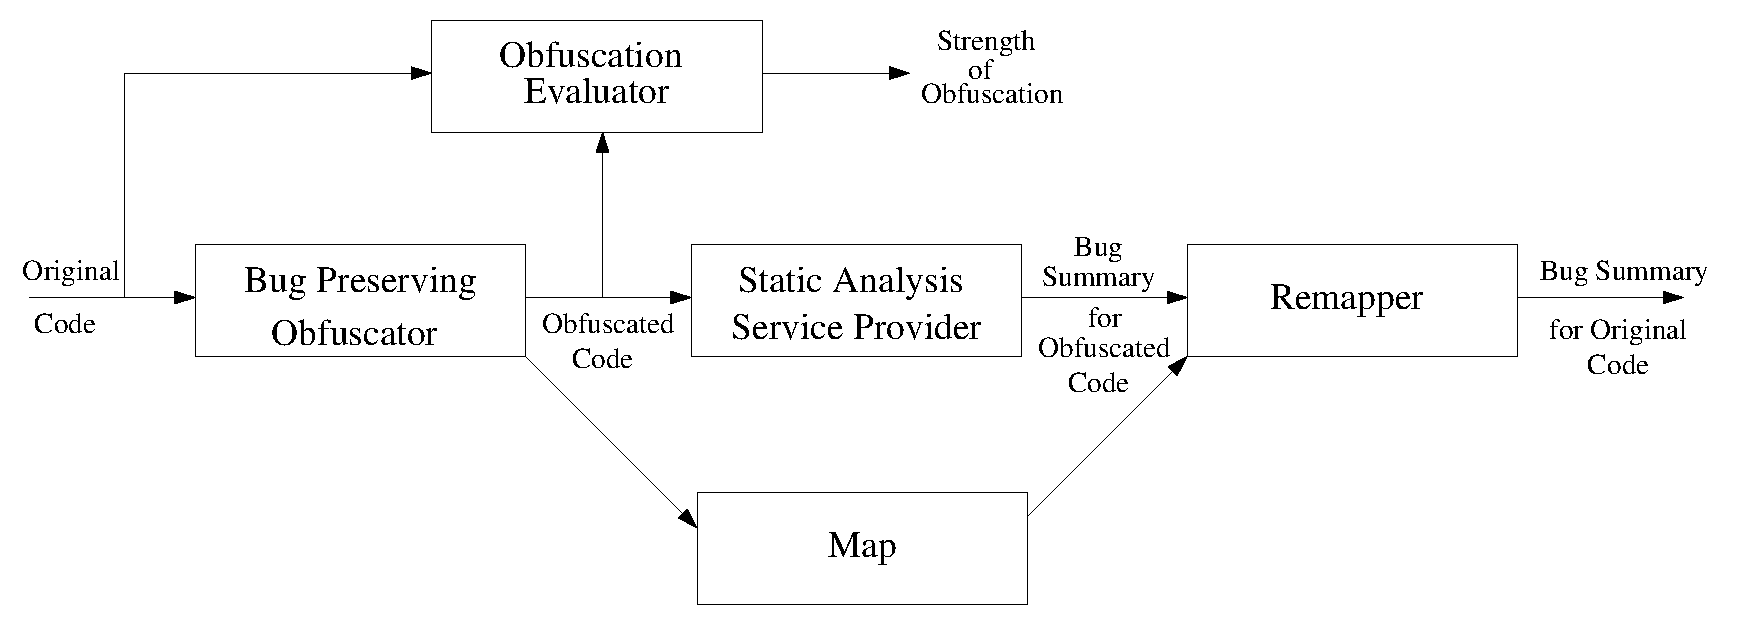
\includegraphics[scale=0.3]{./architecture1.eps}
 % architecture.eps: 0x0 pixel, 300dpi, 0.00x0.00 cm, bb=
 \caption{Architecture of Privacy Preserving Static Analysis System}
 \label{fig:architecture}
\end{figure}

{\tt Bug Preserving Obfuscator} takes as input the original unobfuscated source code and applies certain obfuscation techniques to produce an obfuscated version of the source code, which 
ensures that no new bugs are introduced and none of the old bugs are missing in the obfuscated code. During this obfuscation process our tool also produces a {\tt Map} which maintains a 
mapping of obfuscated package, class, method and variable names to their original ones. The map also stores the full classpath for each and every item in case of repackaging of classes 
or inner classes being moved out of their outer classes. For our tool we use {\tt Proguard Obfuscator} \cite{proguard} as the basis for all 
obfuscation techniques applied. We modify the existing obfuscatation techniques within Proguard to guarantee the preservation of bugs.

The obfuscated code is then sent to the {\tt Static Analysis Service Provider}. The analysis provider runs several static analysis techniques on the obfuscated code and reports back a 
list of found bugs and defects. At this stage even if someone tries to decompile the received code, it is very hard for him to deobfuscate the obfuscated code. For the purpose of our 
tool and testing we have used {\tt FindBugs} \cite{findbugs} as a static analyser. It reports the discovered bugs in a xml format.

The bug summary for the obfuscated code is then sent back to the sender, where it is passed through the {\tt Remapper}. The {\tt Remapper} remaps the bugs in the obfuscated code to 
the respective bugs in the original code. It does so by using the contents of the {\tt Map} produced during the obfuscation phase, and then replaces each obfuscated name, line number 
and classpath with their corresponding original ones. In the end it produces the bug summary for the original code. In our tool the remapper takes FindBugs obfuscated report in xml 
format and outputs the report for original code also in xml format.

Another essential part of the tool is the {\tt Obfuscation Evaluator}. It takes as input both the original and obfuscated code and then measures the strength of obfuscation. The tool 
creates the program dependency graph for both the original and obfuscated program, say $G$ and $G'$ respectively. Now using approximation algorithms for solving {\tt Graph Minor} 
\cite{graphminor} problem, it calculates the cost of transforming $G'$ to $G$. This cost gives an estimate of the cost of reverse engineering, and in turn gives a measure for the 
strength of code obfuscation. We explain {\tt Obfuscation Evaluator} in detail in the next subsection.
\subsection{Measurement of Obfuscation}
In this section we are going to explain in detail the proposed method for measuring the strength of obfuscation including the logic behind it, using examples and step by step procedure 
for calculating the strength of obfuscatation. We can represent any program using a {\tt Program Dependence Graph}, which represents both control and data dependencies. Any obfuscation 
technique increases the complexity level of control flow and data dependencies, and any reverse engineering process tries to simplify them. Therefore it seems very natural to argue about 
the strength of obfuscation using program dependence graph. So in terms of dependence graphs the process of reverse engineering can be seen as a transformation of the obfuscated dependence 
graph to the original dependence graph. We will show this using the following example.
\lstset{language=Java,captionpos=b,caption={Original Code for squaring},label=prog:origsqr}
\tiny\begin{lstlisting}[frame=single]
 int square(int x){
	  int n;
	  n = x * x;
	  return n;
  }
\end{lstlisting}
\normalsize
\lstset{language=Java,captionpos=b,caption={Obfuscated Code for squaring},label=prog:obfsqr}
\tiny\begin{lstlisting}[frame=single]
 int strvup(int m){
	  int o;
	  int i=0;
	  int s=0;
	  while(i < m){
		   s = s + m;
		   i = i + 1;
	  }
	  o = s;
	  return s;
 }
\end{lstlisting}
\normalsize
Listing \ref{prog:origsqr} represents a code to calculate the square of a number and Listing \ref{prog:obfsqr} represents the obfuscated version of it. The corresponding program dependency 
graphs are shown in Figure \ref{fig:origsqr} and Figure \ref{fig:obfsqr1}.
\begin{figure}[h]
 \centering
 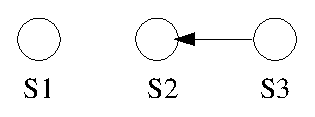
\includegraphics[scale=0.3]{./origdep.eps}
 % architecture.eps: 0x0 pixel, 300dpi, 0.00x0.00 cm, bb=
 \caption{Program dependence graph for Listing \ref{prog:origsqr}}
 \label{fig:origsqr}
\end{figure}
\begin{figure}[h]
 \centering
 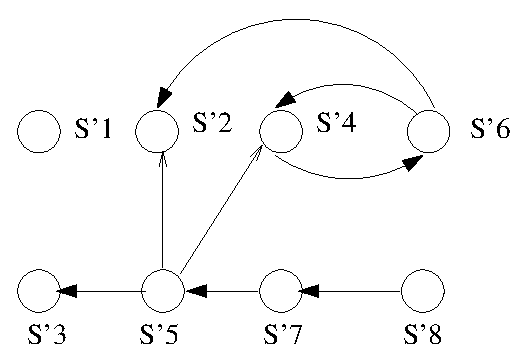
\includegraphics[scale=0.3]{./obfdep1.eps}
 % architecture.eps: 0x0 pixel, 300dpi, 0.00x0.00 cm, bb=
 \caption{Program dependence graph for Listing \ref{prog:obfsqr}}
 \label{fig:obfsqr1}
\end{figure}

Transforming the graph in Figure \ref{fig:obfsqr1} to that in Figure \ref{fig:origsqr} requires a series of operations such as: {\tt edge and node deletion}, and {\tt edge contraction}. 
The sequence of steps needed are shown in Figures \ref{fig:obfsqr2} to \ref{fig:obfsqr7}.
\begin{figure}[ht!]
 \centering
 \subfigure[Step 1]{
        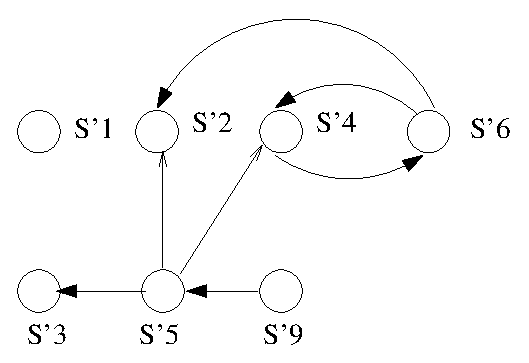
\includegraphics[scale=0.28]{./obfdep2.eps}
	\label{fig:obfsqr2}
 }
 \subfigure[Step 2]{
        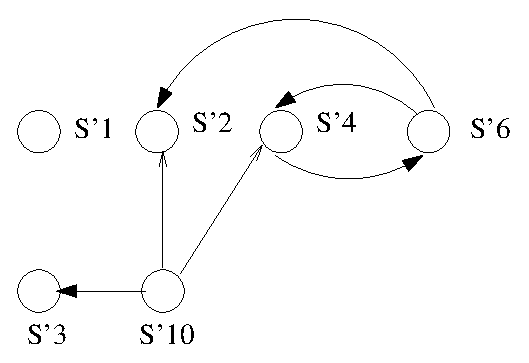
\includegraphics[scale=0.28]{./obfdep3.eps}
	\label{fig:obfsqr3}
 }
 \subfigure[Step 3]{
        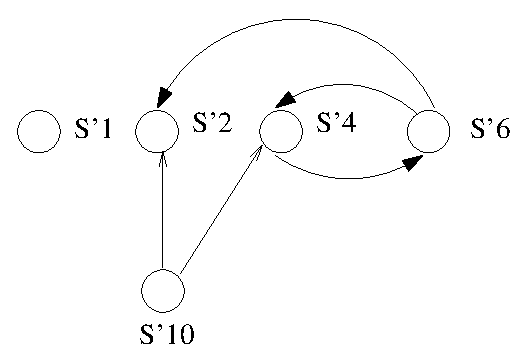
\includegraphics[scale=0.28]{./obfdep4.eps}
	\label{fig:obfsqr4}
 }
 \\
 \subfigure[Step 4]{
        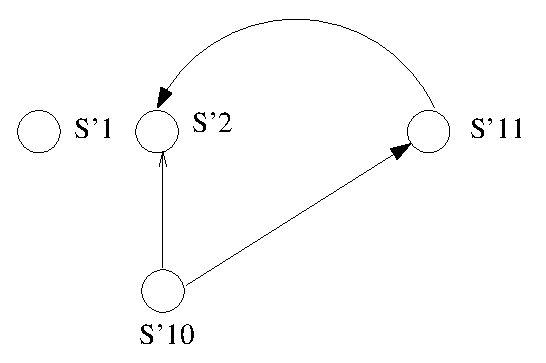
\includegraphics[scale=0.3]{./obfdep5.eps}
	\label{fig:obfsqr5}
 }
 \subfigure[Step 5]{
        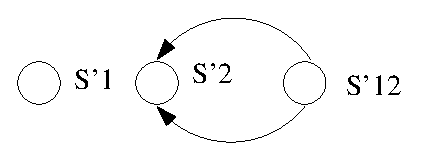
\includegraphics[scale=0.3]{./obfdep6.eps}
	\label{fig:obfsqr6}
 }
 \subfigure[Step 6]{
        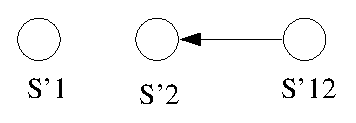
\includegraphics[scale=0.3]{./obfdep7.eps}
	\label{fig:obfsqr7}
 }
\caption{Transformation Steps}
\label{fig:transfrm}
\end{figure}
From Figures \ref{fig:obfsqr2} to \ref{fig:obfsqr7} we see that 4 edge contractions and 2 edge and node deletion is required. During the process of reverse engineering we see that merging 
of two statements is more costlier than deletion of a statement. Hence we can assign higher weightage to edge contraction operations in comparison to edge and node deletion operations. 
We assign each edge contraction operation a weight of 2 and each edge and node deletion operation a weight of 1. Using these weights the cost of reverse engineering or analogously the 
strength of obfuscatation is: $4 * 2 + 2 * 1 = 10$.
% \begin{figure}[h]
%  \centering
%  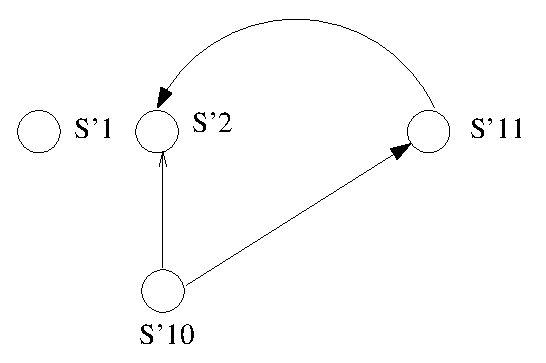
\includegraphics[scale=0.3]{./obfdep5.eps}
%  % architecture.eps: 0x0 pixel, 300dpi, 0.00x0.00 cm, bb=
%  \caption{Step 4}
%  \label{fig:obfsqr5}
% \end{figure}
% \begin{figure}[h]
%  \centering
%  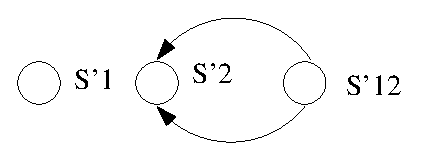
\includegraphics[scale=0.3]{./obfdep6.eps}
%  % architecture.eps: 0x0 pixel, 300dpi, 0.00x0.00 cm, bb=
%  \caption{Step 5}
%  \label{fig:obfsqr6}
% \end{figure}
% \begin{figure}[h]
%  \centering
%  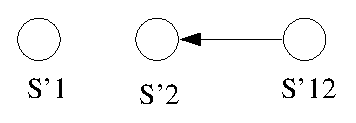
\includegraphics[scale=0.3]{./obfdep7.eps}
%  % architecture.eps: 0x0 pixel, 300dpi, 0.00x0.00 cm, bb=
%  \caption{Step 6}
%  \label{fig:obfsqr7}
% \end{figure}
This method of transforming one graph to another can be mapped to a very popular problem in Graph Theory, known as Graph Minor \cite{graphminor}. Dtermining the steps required for the 
transformation to find the Graph Minor is a NP-Complete problem. But there exist approximation algorithms \cite{Demaine05} for this, using which we can get the approximate steps required. 
Once we have knowledge of these steps, we can then calculate the strength of obfuscatation using the above weights for any pair of original and obfuscated code.
\section{Related Works}
The concept of Privacy Preserving Static Analysis and the idea of providing static analysis is completely new and as such there has been no prior work in this field. The work closest 
to our own is CryptDB project \cite{cryptdb}, which is in the field of database systems. CryptDB uses homomorphic encryption to run queries securely on relational databases. It encrypts 
the data in all possible encryption schemes, layered on top of each other. A trusted proxy stands between clients and database system, analyses the SQL queries on the fly, and decrypts 
the relevant data columns to the right encryption layers so that the query can be executed. In the field of program analysis, MrCrypt \cite{mrcrypt} uses the similar concept of homomorphic 
encryption to securely execute programs on cloud servers without revealing input data. MrCrypt performs type inferencing on a program to identify the set of operations on each input data 
column, in order to select an appropriate homomorphic encryption scheme for that column. It then encrypts the data column and transforms the program to operate over encrypted data. The 
encrypted data and transformed program are uploaded to the server and executed as usual, and the encrypted result of the computation is decrypted on the client side. Both of these 
approaches concentrate on encrypting program data rather than hiding the program structure itself. Moreover the idea of encryption can not be applied for securing program structures as 
it is not possible to run static analysis on encrypted program semantics. So in our proposed method of Privacy Preserving Static Analysis, obfuscation of code successfuly hides program 
structure without caring about program data, while keeping the program semantics unchanged.

There has been substantial work in using static analysis to find bugs in programs. Dillig et al. \cite{dillig} propose a precise technique for a path-sensitive and context-sensitive 
program analysis. Das et al. \cite{das} present an approach for partial program verification in polynomial time. Engler et al. \cite{engler} propose an approach for writing system-specific 
compiler extensions that automatically checks the code for rule violations. This is in contrast to writing abstract specifications that are then verified by model checkers like SPIN 
\cite{spin} or theorem provers like Z3 \cite{z3}. Today several tools exist in the market which provide static analysis to detect bugs \cite{coverity,klocwork,parasoft,findbugs,chess,saturn}. 
Coverity \cite{billionlinesofcode} was the first to commercialize a static analysis tool for bug detection. FindBugs \cite{findbugs} uses bug pattern detectors to find real bugs in 
several real world Java applications and libraries. Our tool works considering FindBugs as the static analysis tool. But any other bug detecting tool would have worked fine, since in 
our tool we modified the obfuscatation techniques based on certain properties of bug checkers which are same for most other static analysis tools.

Even in the field of Code Obfuscation there has been quite a lot prior works. A theoretical approach to obfuscations was presented by Collberg et al. \cite{collberg}. They introduce 
the concepts of lexical obfuscations (name changing) and data transformations (e.g., splitting boolean values into two discrete numerics that are combined only at evaluation time). 
However, their chief contributions are in control-flow obfuscations. They make use of opaque predicates to introduce dead code, specifically engineering the dead branches to have buggy 
versions of the live branches. A technique for combining the data of a program with its control-flow was developed by Wang et al. \cite{wang}, whereby control and data flow analysis become 
codependent. Sakabe et al. \cite{sakabe} concentrate their efforts on the object-oriented nature of Java — the high-level information in a program. Using polymorphism, they invent a 
unique return type class which encapsulates all return types and then modify every method to return an object of this type. Unfortunately, their empirical results show significantly 
slower execution speeds — an average slowdown of $30\%$ — and a $300\%$ blowup in class file size. Sonsonkin et al. \cite{sonsonkin} attempt to confuse program structure by suggesting the coalescing of 
multiple class files into one. For our tool we are building on top of Proguard Obfuscator tool \cite{proguard}.

Although there have been several works related to code obfuscation but unfortunately there are no sufficient or satisfactory work for measuring obfuscation strength. Collberg et al. 
\cite{collberg} measures potent and resilient opaque predicates but in a qualitative way. Some other measures of program obfuscatation can relate to instruction count, data-flow, 
control-flow as distinguished in \cite{sutter} or it may be cyclomatic complexity as mentioned in \cite{McCabe}. Most of the prior works measure code obfuscatation qualitatively rather 
than quantitatively. A very recent work \cite{entropy} suggests measuring the entropy of an obfuscated code, but unfortunately it only deals with control flow obfuscatations. We deal 
with these problems in our proposed method by representing programs as program dependence graphs, and then draw an analogy between reverse engineering and transformation of obfuscated 
dependence graph to original dependence graph. Although this is a NP-Complete problem, but there exist some approximation algorithms such as \cite{Demaine05}. Using these approximation 
algorithms we can compute the approximate cost of reverse engineering.
%%%%%%%%%%%%%  This can be followed by several other sections
\section{Conclusions}
We present the notion of Privacy Preserving Static Analysis System and the design for its implementation. The project is the first of its kind to define static analysis as a service, 
but at the same time it also preserves the privacy of the analysed programs. We also propose a measure for calculating and comparing the strength of obfuscated codes, which gives the 
true cost of reverse engineering. We will implement all these as a part of a tool which takes a program as input and outputs the obfuscated version of it such that, it preserves all 
the defects. The tool will also report a value indicating the strength of the obfuscated code. The effectiveness of the tool will be verified by running it on the three large benchmark 
programs.
{
 \bibliographystyle{plain}
 \bibliography{citation}
}

% \begin{thebibliography}{1}
%
%\bibitem{IEEEhowto:kopka}
%H.~Kopka and P.~W. Daly, \emph{A Guide to \LaTeX}, 3rd~ed.\hskip 1em plus
%  0.5em minus 0.4em\relax Harlow, England: Addison-Wesley, 1999.
%  
%
%\end{thebibliography}



% that's all folks
\end{document}


